As mentioned in the previous section a strictly interactive evolutionary approach was not adhered to: there were a few tools at the disposal of the operators. However the initial results somewhat necessitated these changes, an observation that will be described shortly. Figures \ref{fig:bigeye} to \ref{fig:color_extraction} show four examples of interesting distortion generated in the evolutionary process.

\begin{figure*}
    \centering
    \subfigure[]{
        \label{fig:bigeye:network}
        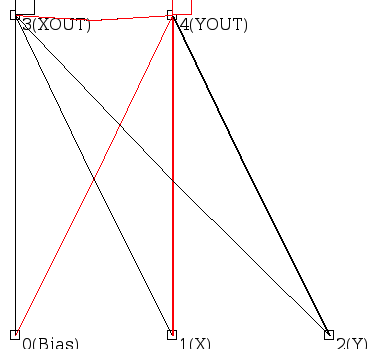
\includegraphics[height=2in]{../../rec/networks/bigeye_13.png}
    } \\
    \subfigure[]{
        \label{fig:bigeye:arnold}
        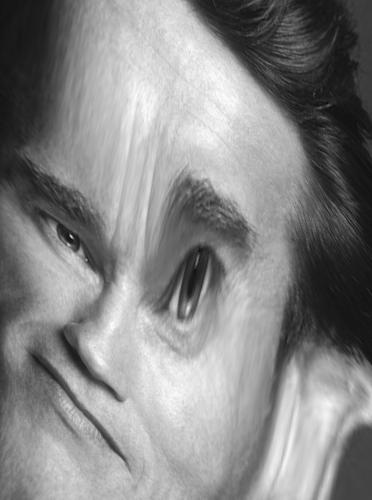
\includegraphics[height=1.8in]{../../rec/faces_distorted/bigeye_13_arnold_schwarzenegger.jpg}
    }
    \subfigure[]{
        \label{fig:bigeye:michael}
        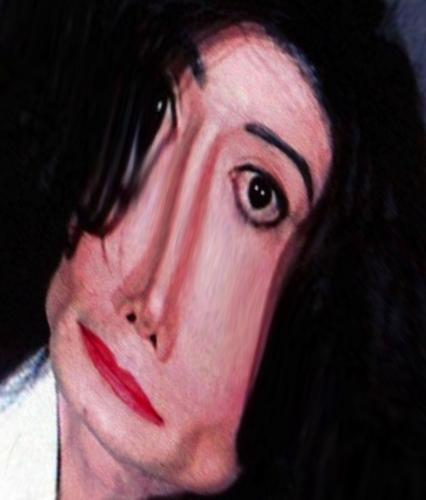
\includegraphics[height=1.8in]{../../rec/faces_distorted/bigeye_13_michael_jackson.jpg}
    } \\
    \subfigure[]{
        \label{fig:bigeye:old_man}
        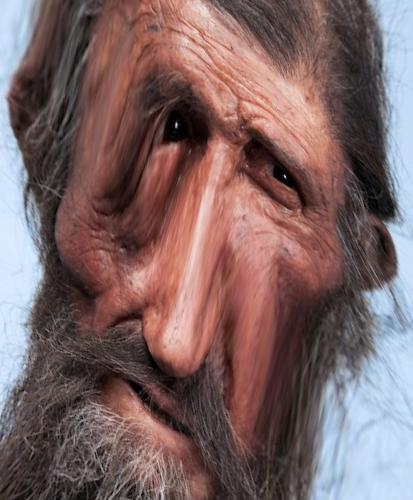
\includegraphics[height=1.8in]{../../rec/faces_distorted/bigeye_13_old_man.jpg}
    }
    \subfigure[]{
        \label{fig:bigeye:mona_lisa}
        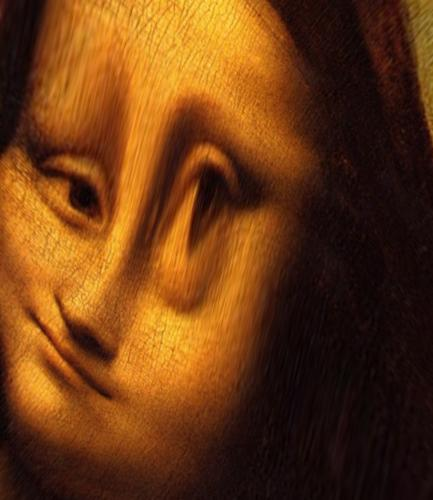
\includegraphics[height=1.8in]{../../rec/faces_distorted/bigeye_13_mona_lisa.jpg}
    } \\
    \subfigure[]{
        \label{fig:bigeye:spongebob}
        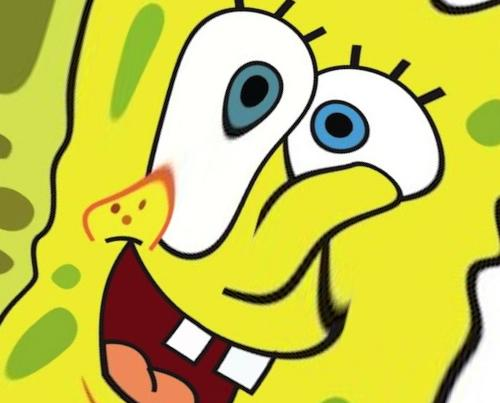
\includegraphics[height=1.8in]{../../rec/faces_distorted/bigeye_13_spongebob.jpg}
    }
    \caption{Big-eye distortion: \ref{fig:bigeye:network} the network and \ref{fig:bigeye:arnold}-\ref{fig:bigeye:spongebob} the distorted face set.\label{fig:bigeye}}
\end{figure*}

\begin{figure*}
    \centering
    \subfigure[]{
        \label{fig:multieye:network}
        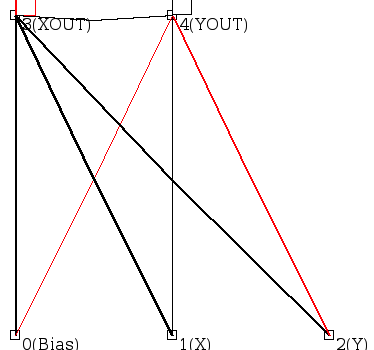
\includegraphics[height=2in]{../../rec/networks/multieye_1.png}
    } \\
    \subfigure[]{
        \label{fig:multieye:arnold}
        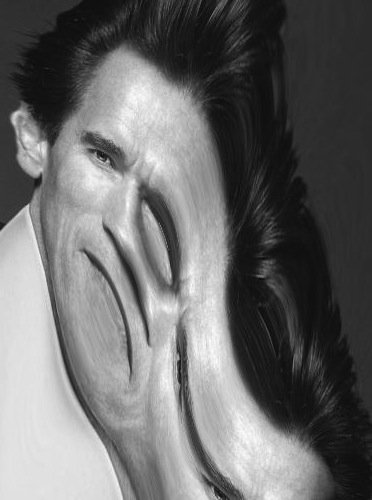
\includegraphics[height=1.8in]{../../rec/faces_distorted/multieye_1_arnold_schwarzenegger.jpg}
    }
    \subfigure[]{
        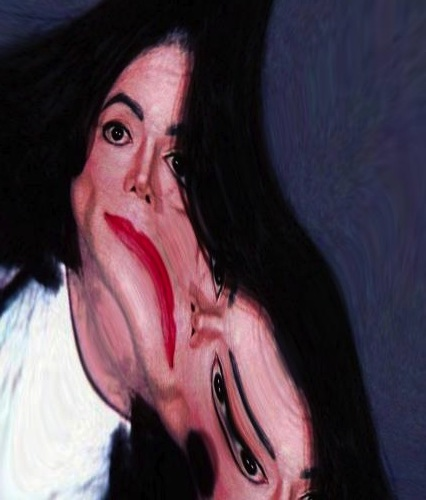
\includegraphics[height=1.8in]{../../rec/faces_distorted/multieye_1_michael_jackson.jpg}
    } \\
    \subfigure[]{
        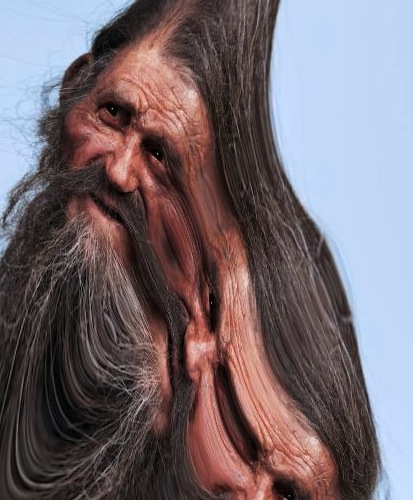
\includegraphics[height=1.8in]{../../rec/faces_distorted/multieye_1_old_man.jpg}
    }
    \subfigure[]{
        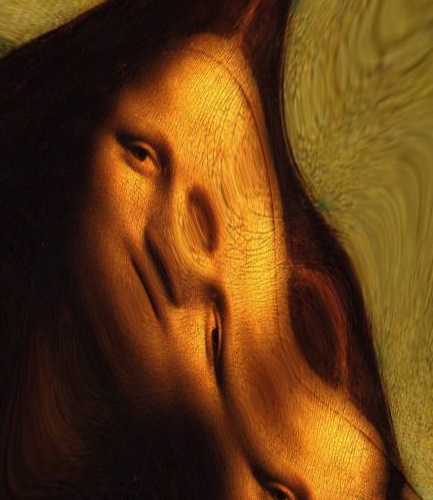
\includegraphics[height=1.8in]{../../rec/faces_distorted/multieye_1_mona_lisa.jpg}
    } \\
    \subfigure[]{
        \label{fig:multieye:spongebob}
        
\includegraphics[height=1.8in]{../../rec/faces_distorted/multieye_1_spongebob.jpg}
    }
    \caption{Multi-eye distortion: \ref{fig:multieye:network} the network and \ref{fig:multieye:arnold}-\ref{fig:multieye:spongebob} the distorted face set.\label{fig:multieye}}
\end{figure*}

\begin{figure*}
    \centering
    \subfigure[]{
        \label{fig:gauss_v:network}
        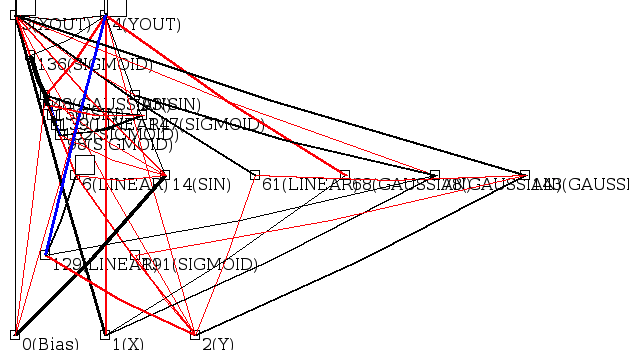
\includegraphics[height=2in]{../../rec/networks/gauss_v_12.png}
    } \\
    \subfigure[]{
        \label{fig:gauss_v:arnold}
        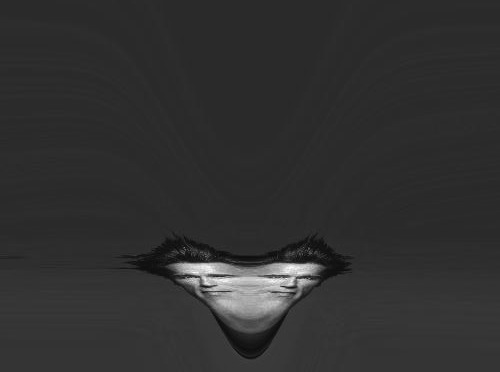
\includegraphics[height=1.8in]{../../rec/faces_distorted/gauss_v_12_arnold_schwarzenegger.jpg}
    }
    \subfigure[]{
        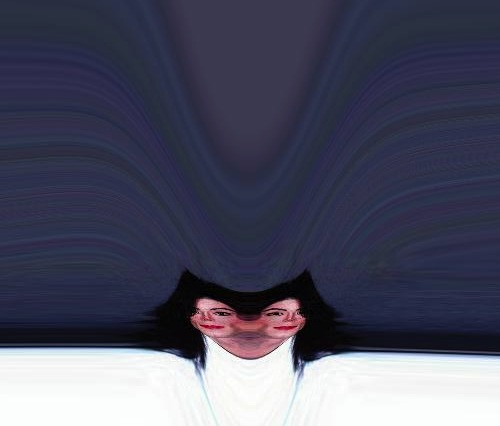
\includegraphics[height=1.8in]{../../rec/faces_distorted/gauss_v_12_michael_jackson.jpg}
    } \\
    \subfigure[]{
        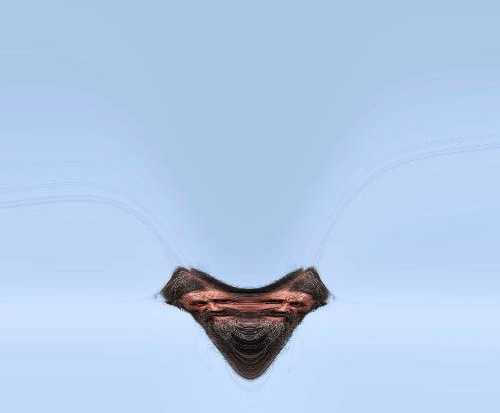
\includegraphics[height=1.8in]{../../rec/faces_distorted/gauss_v_12_old_man.jpg}
    }
    \subfigure[]{
        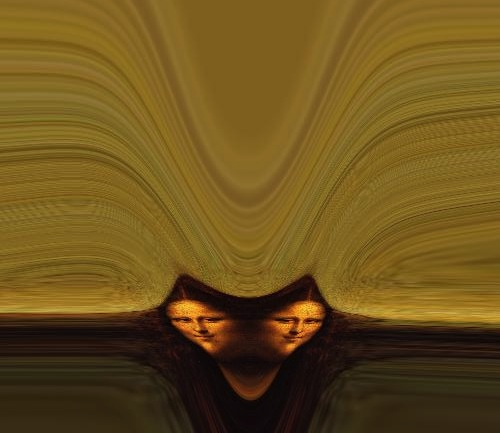
\includegraphics[height=1.8in]{../../rec/faces_distorted/gauss_v_12_mona_lisa.jpg}
    } \\
    \subfigure[]{
        \label{fig:gauss_v:spongebob}
        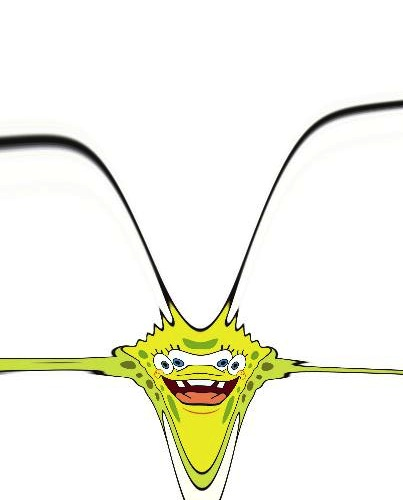
\includegraphics[height=1.8in]{../../rec/faces_distorted/gauss_v_12_spongebob.jpg}
    }
    \caption{Gaussian V distortion: \ref{fig:gauss_v:network} the network and \ref{fig:gauss_v:arnold}-\ref{fig:gauss_v:spongebob} the distorted face set.\label{fig:gauss_v}}
\end{figure*}

\begin{figure*}
    \centering
    \subfigure[]{
        \label{fig:color_extraction:network}
        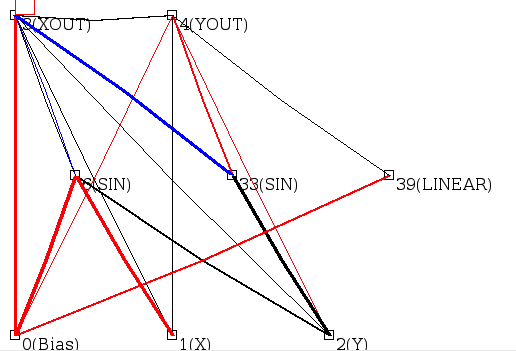
\includegraphics[height=2in]{../../rec/networks/spongebob__colors_extracted__13.png}
    } \\
    \subfigure[]{
        \label{fig:color_extraction:arnold}
        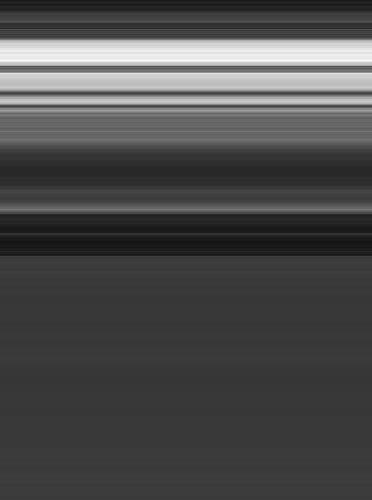
\includegraphics[height=1.8in]{../../rec/faces_distorted/spongebob__colors_extracted__13_arnold_schwarzenegger.jpg}
    }
    \subfigure[]{
        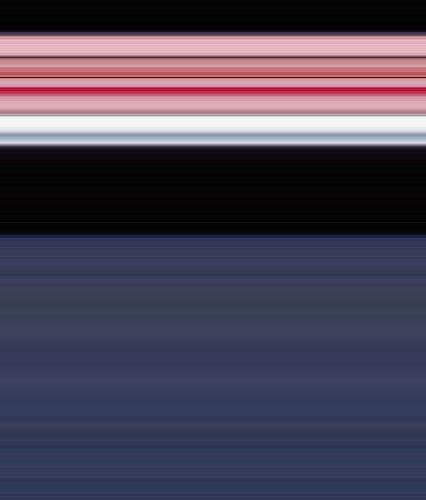
\includegraphics[height=1.8in]{../../rec/faces_distorted/spongebob__colors_extracted__13_michael_jackson.jpg}
    } \\
    \subfigure[]{
        
\includegraphics[height=1.8in]{../../rec/faces_distorted/spongebob__colors_extracted__13_old_man.jpg}
    }
    \subfigure[]{
        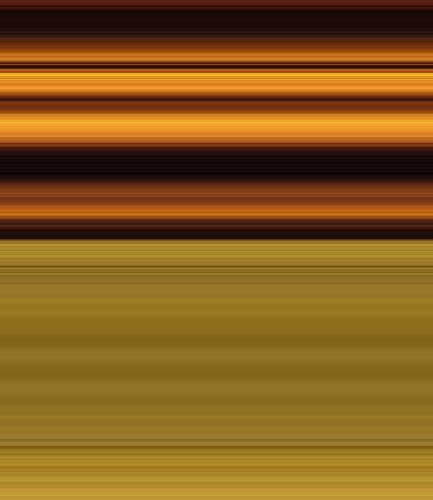
\includegraphics[height=1.8in]{../../rec/faces_distorted/spongebob__colors_extracted__13_mona_lisa.jpg}
    } \\
    \subfigure[]{
        \label{fig:color_extraction:spongebob}
        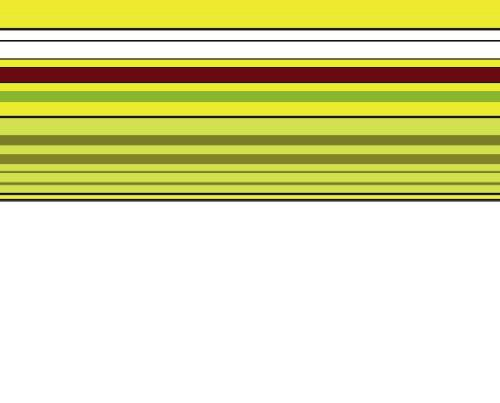
\includegraphics[height=1.8in]{../../rec/faces_distorted/spongebob__colors_extracted__13_spongebob.jpg}
    }
    \caption{Color extraction distortion: \ref{fig:color_extraction:network} the network and \ref{fig:color_extraction:arnold}-\ref{fig:color_extraction:spongebob} the distorted face set.\label{fig:color_extraction}}
\end{figure*}

Figures \ref{fig:bigeye} and \ref{fig:multieye} are examples of interesting distortions attained prior to the implementation of the boosting process. The first, the ``big eye'' distortion, creates an odd elongation of the eye. This is one of the cases mentioned previously where the results, while performing the same operation, yield different artifacts per each image. Notice on figures \ref{fig:bigeye:arnold}, \ref{fig:bigeye:michael}, and \ref{fig:bigeye:mona_lisa} it would appear that each individual's left eye is elongated, though on \ref{fig:bigeye:old_man} and \ref{fig:bigeye:spongebob} it would appear to be the right. Just given the different head geometry and orientation the essence of what distortion is taking place is fundamentally altered. This is something which could perhaps be fixed by first warping the image into a predefined coordinate space which will be discussed later.

Figures \ref{fig:multieye:arnold} to \ref{fig:multieye:spongebob}, victims of the ``multi-eye`` distortion, are very interesting for a few reasons. First, in general it's a quite odd warping that has occurred. The face of the individuals seems repeated and warped in a very fluid manner yielding nicely connected mouths and sets of eyes. It's oddly comforting to see the features flow together to form a face that could be somewhat realistic, though far-fetched, with it's flowing hairlines and its oddly shaped but not completely disjoint features. But what seems most interesting here is the warping to the cartoon character \ref{fig:multieye:spongebob}. It wasn't surprising to see the combination of multiple faces in the same weaving fashion observed in the other images. What was surprising is the seeming lack of blending and well defined features. On the lower three-eyed face, for example, it was not at all expected that the eyes would be three independent clearly defined eyes as opposed to a blur as in the other faces. This is a feature consistent across all distortions of the cartoon which seems to be primarily due to the limited palette used in the image so very little blurring actually occurs. This has two interesting applications: first, the face evolution can probably be used with great success to form new cartoon character morphs because definition is maintained and limited blurring occurs; second, a realistically proportioned cartoon of a face can be used to see with greater ease exactly what the distortion is accomplishing, which might be useful in the search for generic interesting distortions.

The last two distortions seemed fairly interesting. The issue prior to incorporating the boosting though was that complexity didn't grow very well without a large number of generations. Even with a number of generations many interesting networks had little or no hidden nodes (the previous distortion networks figures \ref{fig:bigeye:network} and \ref{fig:multieye:network} had none). As long as interesting distortions come out this isn't a huge issue but the lack of complexity was yielding a constrained set of distortions that reappeared on a run to run basis. The first resort was to meddle with the complexifying evolution parameters (node and link creation) but this resulted in quite a bit of parameter ''thrashing`` as the parameters would need to be modified sufficiently high or low to provoke or inhibit complexification. The boosting method seemed to offer a good approach allowing rapid complexification when needed and fine tuned adjustments when it wasn't needed.

The distortions represented in figures \ref{fig:gauss_v} and \ref{fig:color_extraction} are more complex examples. By comparing their networks (figures \ref{fig:gauss_v:network} and \ref{fig:color_extraction:network}) with those of the last two examples (figures \ref{fig:bigeye:network} and \ref{fig:multieye:network}) the complexity difference is obvious. It's also obvious when evaluating the distortions that arise as a result.

Figure \ref{fig:gauss_v}, the ''Gaussian V``, has a quite large network for a distortion that seems fairly fluent and not terribly difficult to explain. For the real faces and the painting it pretty consistently spits out a two headed amalgam backed by a very interesting ''V`` shaped texture. Again, what's really interesting though is the cartoon figure where the distortion, due potentially to the lack of refined detail and the exaggerated features, generates something more a kin to a new creature than the old one somewhat warped. The cartoon has turned in to some sort of bug or alien creature. This is a perception that's completely different than what's gathered from the same distortion applied to the other images.

The final distortion depicted in figure \ref{fig:color_extraction} is a fairly simple network that creates from an image of a face a linear texture using the colors extracted from the original image. Some how this network seems to have grabbed a single column from the original image, flipped the upper and lower halves, stretched one and compressed the other, then tiled it across the image. This is done with two sine nodes and one linear node. It's a pretty interesting outcome that doesn't seem at all intuitive given the network. It does serve to demonstrate the inherent difficulty in understanding CPPNs based purely on their makeup, even simple CPPNs with three hidden nodes.